%==============================================================================
% Sjabloon poster bachproef
%==============================================================================
% Gebaseerd op document class `a0poster' door Gerlinde Kettl en Matthias Weiser
% Aangepast voor gebruik aan HOGENT door Jens Buysse en Bert Van Vreckem

\documentclass[a0,portrait]{hogent-poster}
\usepackage{graphicx}
% Info over de opleiding
\course{Bachelorproef}
\studyprogramme{toegepaste informatica}
\academicyear{2023-2024}
\institution{Hogeschool Gent, Valentin Vaerwyckweg 1, 9000 Gent}

% Info over de bachelorproef
\title{De beste JavaScript runtime-omgeving voor performante applicaties: een vergelijkende studie}
% \subtitle{Ondertitel (eventueel)}
\author{Quinten De Wolf}
\email{quinten.dewolf2@student.hogent.be}
\supervisor{Martine Van Audenrode}
\cosupervisor{Dmitriy Van Der Elst (Cognit bv. - Involv Intranet)}

% Indien ingevuld, wordt deze informatie toegevoegd aan het einde van de
% abstract. Zet in commentaar als je dit niet wilt.
\specialisation{Mobile en Enterprise development}
\keywords{Bun, Node.js, backend}
\projectrepo{https://github.com/user/repo}

\begin{document}

\maketitle

\begin{abstract}
Er worden voortdurend nieuwe JavaScript runtime-omgevingen ontwikkeld met telkens nieuwe verbeteringen. 
Echter worden weinig van deze nieuwe ontwikkelingen effectief in de praktijk gebruikt.
Zo is het oudere Node.js nog altijd de standaard in de industrie. 
In dit onderzoek wordt inzicht verschaft in de performantie van Node.js en één van deze nieuwe omgevingen 
om zo een geschikte keuze te kunnen maken bij de ontwikkeling van performante JavaScript applicaties.
Aan de hand van een requirements analyse werd gekozen om Bun te vergelijken met Node.js.
Voor deze vergelijking werden proof-of-concepts gemaakt voor beide omgeving waarop performantie metingen werden uitgevoerd.
Het resultaat toont aan dat Bun een optimale keuze blijkt te zijn voor applicaties met complexe algoritmes en calculaties door de snellere uitvoeringstijd.
Daarnaast presteert Bun beter bij I/O-taken, zoals het verwerken van verzoeken en het verminderen van latentie. Dit gaat echter gepaard met een hoger middelengebruik.
Hierbij moet dus de afweging gemaakt worden tussen de snellere verwerking van Bun en het hogere middelengebruik dat hiermee gepaard gaat.
\end{abstract}

\begin{multicols}{2} % This is how many columns your poster will be broken into, a portrait poster is generally split into 2 columns

\section{Introductie}
Node.js is nog altijd de standaard keuze bij JavaScript runtime-omgevingen. 
Er zijn echter tal van andere omgevingen die kunnen voldoen aan de specifieke behoeften waar Node.js tekortschiet.
Zo is de nood aan goede performantie doorheen de tijd alsmaar belangrijker geworden voor JavaScript backend applicaties.
Bun probeert hierop in te spelen door een performantere omgeving aan te bieden. 
In dit onderzoek wordt dieper ingegaan op deze performantie en wordt deze vergeleken met Node.js.
Op basis van de resultaten kan een weloverwogen keuze gemaakt worden bij de ontwikkeling van performante JavaScript backend applicaties.
Specifiek worden aan de hand van de metingen bij de proof-of-concepts volgende vragen beantwoord:
\begin{itemize}
  \item Wat zijn de onderliggende verschillen tussen Node.js en Bun?
  \item Is Bun performanter dan Node.js bij het uitvoeren van computationele berekeningen?
  \item Is Bun performanter dan Node.js bij het afhandelen van netwerkverzoeken?
  \item Wat is het verschil tussen hun respectievelijke package managers?
\end{itemize}
\section{Experimenten}
\begin{center}
  \captionsetup{type=figure}
  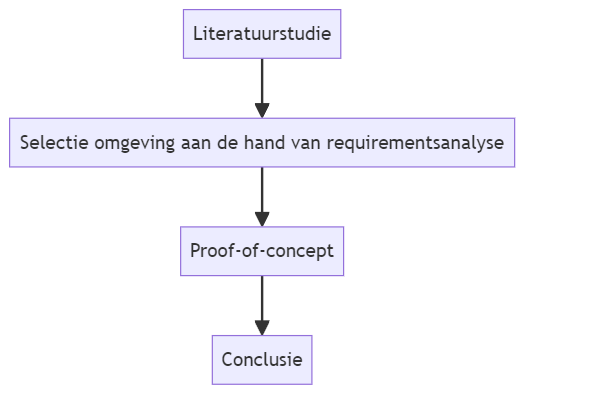
\includegraphics[width=0.7\linewidth]{flowchart}
  \captionof{figure}{Flowchart van de methodologie}
\end{center}
Het onderzoek bevat 4 fasen. 
In de eerste fase wordt een beter begrip over de JavaScript runtime-omgevingen en het onderzoeksdomein bekomen aan de hand van een literatuurstudie.
In de tweede fase wordt, aan de hand van een requirementsanalyse, één omgeving geselecteerd om de performantie te vergelijken met Node.js.
In de derde fase worden de zelfgemaakte proof-of-concepts opgesteld en getest voor beide omgevingen. 
Hierbij wordt een applicatie ontwikkeld waarbij een gebruiker onderwerpen kan ophalen en beoordelen, alsook een script dat het QuickSort algoritme uitvoert.
De metingen worden uitgevoerd met behulp van 2 benchmark tools, Hyperfine en Bombardier, om volgende zaken te kunnen meten:
\begin{itemize}
    \item De latentie van de applicatie.
    \item Het aantal verzoeken per seconde bij de applicatie.
    \item De uitvoeringstijd van de berekeningen van het QuickSort algoritme.
    \item Het geheugengebruik bij de applicatie.
    \item De installatietijd voor de respectievelijke package managers.
    \item Het CPU-gebruik bij de applicatie.
\end{itemize}
Bij de applicatie worden de metingen zowel bij een MySQL databank als bij een PostgreSQL databank uitgevoerd met behulp van een ORM.
Aan de hand van de resultaten komen we tot bij de laatste fase namelijk de conclusie. Hierbij wordt de data geïnterpreteerd om een antwoord te formuleren op de onderzoeksvragen.
Uit deze antwoorden kan afgeleid worden of Bun een geschikte plaatsvervanger kan zijn voor Node.js binnen de ontwikkeling van performantie backend applicaties.
Bij het QuickSort algoritme had Bun een snellere uitvoeringstijd dan Node.js, met name 2.21 keer sneller.
Bij de applicatie scoorde Bun beter bij het ophalen en invoegen van data op vlak van
aantal verzoeken per seconde en latentie maar verbruikte hiervoor wel telkens meer middelen.
\begin{center}
  \captionsetup{type=figure}
  \begin{minipage}{0.20\textwidth}
    \centering
    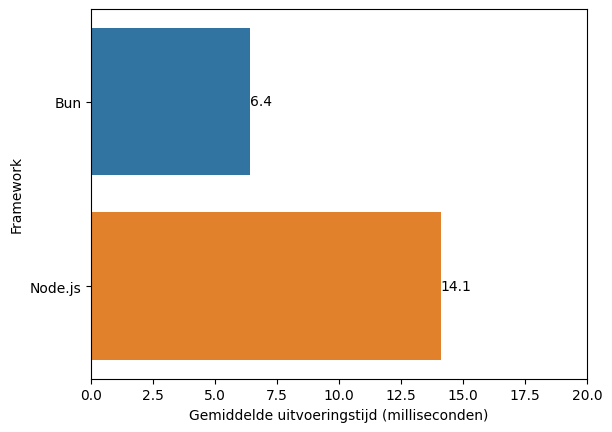
\includegraphics[width=\linewidth]{scriptuitvoeringstijd}
    \caption{Uitvoeringstijd van het QuickSort algoritme}
  \end{minipage}%
  \hfill
  \begin{minipage}{0.20\textwidth}
    \centering
    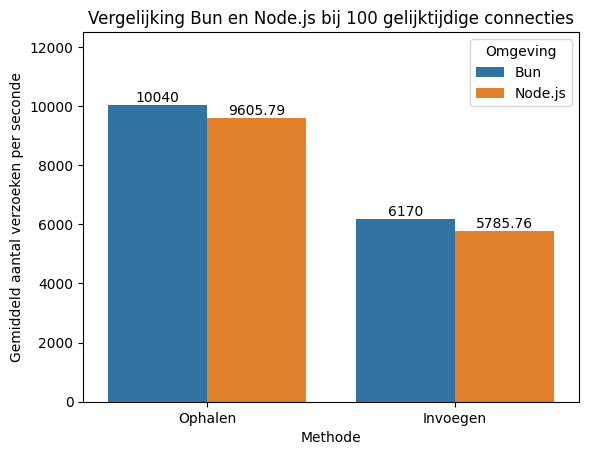
\includegraphics[width=\linewidth]{requests}
    \caption{Visuele voorstelling gemiddeld aantal verzoeken per seconde met PostgreSQL}
  \end{minipage}%
\end{center}
\begin{center}
  \captionsetup{type=figure}
  \begin{minipage}{0.20\textwidth}
    \centering
    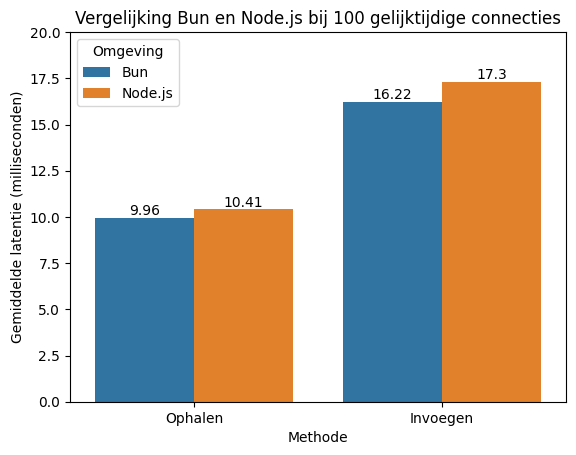
\includegraphics[width=\linewidth]{latentie}
    \caption{Visuele voorstelling gemiddelde latentie met PostgreSQL}
  \end{minipage}%
  \hfill
  \begin{minipage}{0.20\textwidth}
    \centering
    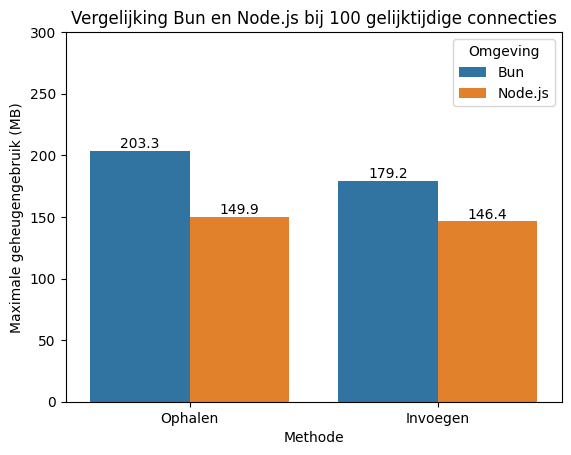
\includegraphics[width=\linewidth]{geheugen}
    \caption{Visuele voorstelling maximale geheugengebruik met PostgreSQL}
  \end{minipage}
\end{center}

\section{Conclusies}
De onderzoeksvraag betreffende de onderliggende verschillen tussen beide omgevingen werd beantwoord door de literatuurstudie.
Zo gebruikt Bun de JavaScriptCore engine die 3 JIT compiler en een Low-Level Interpreter bevat in plaats van de V8 JavaScript engine die Node.js gebruikt.
Bun gebruikt ook Zig als programmeertaal in plaats van C. Deze keuzes zorgen voor een verschil in computationele en I/O performantie tussen beide omgevingen.
Zo tonen de metingen van het QuickSort algoritme aan dat Bun computationeel sneller is dan Node.js. 
Bij de I/O performantie scoort Bun ook beter op vlak het verwerken van verzoeken maar komt dit ten koste van een hoger middelengebruik.
Uit de metingen blijkt Bun een optimale keuze te zijn voor applicaties met complexe algoritmes en calculaties. 
Echter moet bij applicaties met veel I/O-taken een afweging gemaakt worden tussen de snellere verwerking van Bun en het hogere middelengebruik dat hiermee gepaard gaat.
\section{Toekomstig onderzoek}
Toekomstig onderzoek kan verder gaan op de bekomen resultaten door in plaats van relationele databanken ook NoSQL databanken te testen.
Daarnaast werden in dit onderzoek de test runner en bundler van Bun niet vergeleken. Verder onderzoek zou zich hierop kunnen richten om deze te vergelijken met andere alternatieven.

\end{multicols}
\end{document}